\documentclass[11pt]{article}
\usepackage[utf8]{inputenc}    
\usepackage[T1]{fontenc}  
\usepackage{amsmath}   
\usepackage{bm}  
\usepackage{amssymb}
\usepackage{amsmath} 
\usepackage{forest}
\usepackage{tikz}

% Comando \circulo{texto}
\newcommand{\circulo}[1]{%
  \begin{tikzpicture}[baseline=(char.base)]
    \node[shape=circle, draw, inner sep=1.5pt, minimum size=1.5em] (char) {\small #1};
  \end{tikzpicture}%
}

\title{AT2 - Métodos Matemáticos para Gestão da Informação}
\date{}
\author{Juliane Pires}
\begin{document}

\maketitle

% Questão 1
\subsection*{PARTE A — Matrizes como estrutura de dados}
\subsubsection*{1. Considere as matrizes:}
$$
A = \begin{bmatrix}
    2 & 4 \\
    6 & 8
\end{bmatrix}
\qquad 
B = \begin{bmatrix}
    1 & 3 \\
    5 & 7
\end{bmatrix}
$$
\subsubsection*{Calcule:}
%a)
\subparagraph{a) A + B}
$$
\begin{bmatrix}
    2 & 4 \\
    6 & 8
\end{bmatrix}
+ 
\begin{bmatrix}
    1 & 3 \\
    5 & 7
\end{bmatrix}
=
\begin{bmatrix}
    3 & 7 \\
    11 & 15
\end{bmatrix}\\
$$
%b)
\subparagraph{b) A - B}
$$
\begin{bmatrix}
    2 & 4 \\
    6 & 8
\end{bmatrix}
- 
\begin{bmatrix}
    1 & 3 \\
    5 & 7
\end{bmatrix}
=
\begin{bmatrix}
    1 & 1 \\
    1 & 1
\end{bmatrix}
$$
%c)
\subparagraph{c) 2A}
$$
2 \times \begin{bmatrix}
    2 & 4 \\
    6 & 8
\end{bmatrix}
=
\begin{bmatrix}
    4 & 8 \\
    12 & 16
\end{bmatrix}
$$
%d)
\subparagraph{d) A$^T$}
$$
A^T = \begin{bmatrix}
    2 & 6 \\
    4 & 8
\end{bmatrix}
$$

%Questão 2
\subsubsection*{2. Considere a matriz:}
$$
C = \begin{bmatrix}
    5 & 2 & 1 \\
    3 & 6 & 4
\end{bmatrix}
$$
%a)
\subparagraph{a) Informe a ordem da matriz.\\}
A matriz tem 2 linhas e 3 colunas, ou seja, é uma matriz $2\times3\\$.
%b)
\subparagraph{b) Identifique o elemento C$_{23}$.\\}
O elemento C$_{23}$ é o elemento que está na linha 2 e na coluna 3, ou seja, é o $\bm4$.
%c)
\subparagraph{c) Calcule a média da primeira linha.\\}
$(5 + 2 + 1) \div 3 = 8 \div 3 = \bm{2,66}$
%d)
\subparagraph{d) Calcule a amplitude da segunda linha.\\}
A amplitude da segunda linha é o cálculo do maior velor pelo menor valor da linha, ou seja:
$6 - 3 = \bm3$

% Questão 3
\subsection*{PARTE B — Distâncias e Agrupamento Hierárquico (Complete Linkage)}
\subsubsection*{Considere os vetores:}
$
P1 = (1,1)\\
P2 = (2,3)\\
P3 = (6,5)\\
P4 = (7,4)
$
\subsubsection*{3. Matriz de distâncias (Euclidiana)}
\subsubsection*{a) Calcule todas as distâncias Euclidianas entre os pontos.}
$\underset{1,2}{D} = \sqrt{(1-2)^2 + (1-3)^2} = \sqrt{1+4} = \sqrt{5} = \bm{2,23}\\$
$\underset{1,3}{D} = \sqrt{(1-6)^2 + (1-5)^2} = \sqrt{25+16} = \sqrt{41} = \bm{6,40}\\$
$\underset{1,4}{D} = \sqrt{(1-7)^2 + (1-4)^2} = \sqrt{36+9} = \sqrt{45} = \bm{6,70}\\$
$\underset{2,3}{D} = \sqrt{(2-6)^2 + (3-5)^2} = \sqrt{16+4} = \sqrt{20} = \bm{4,47}\\$
$\underset{2,4}{D} = \sqrt{(2-7)^2 + (3-4)^2} = \sqrt{25+1} = \sqrt{26} = \bm{5,09}\\$
$\underset{3,4}{D} = \sqrt{(6-7)^2 + (5-4)^2} = \sqrt{1+1} = \sqrt{2} = \bm{1,41}$
\subsubsection*{b) Construa a matriz de distâncias 4×4.}
% \renewcommand aumenta o espaço entre as linhas
\renewcommand{\arraystretch}{1.5}
$$
\begin{tabular}{|c|c|c|c|c|}
    \hline
    & $P1$ & $P2$ & $P3$ & $P4$ \\ \hline
    $P1$ & 0     & 2,23  & 6,40  & 6,70  \\ \hline
    $P2$ & 2,23  & 0     & 4,47  & 5,09  \\ \hline
    $P3$ & 6,40  & 4,47  & 0     & 1,41  \\ \hline
    $P4$ & 6,70  & 5,09  & 1,41  & 0     \\ \hline
\end{tabular}
$$

% Questão 4
\subsubsection*{4. Agrupamento hierárquico (Complete Linkage)}
\subsubsection*{Utilizando a matriz do exercício anterior:}

%a)
\subsubsection*{a) Identifique o primeiro par agrupado e a respectiva altura.}
O primeiro par agrupado é a menor distância diferente de $\underline{zero}$, ou seja:
$(P3,P4)$, sendo a altura no dendograma $= 1,41$.
% b)
\subsubsection*{b) Construa a matriz reduzida após a primeira fusão.}
\textcircled{1} Calcula-se a distância do novo grupo (P3,P4) em relação aos pontos restantes (P1 e P2):\\\\
$\rightarrow$ Distância de (P3,P4) até P1:\\
$d((P3,P4),P1) = max(d(P3,P1),d(P4,P1)) = max(6,40;6,70) = 6,70$\\\\
$\rightarrow$ Distância de (P3,P4) até P2:\\
$d((P3,P4),P2) = max(d(P3,P2),d(P4,P2)) = max(4,47;5,09) = 5,09$\\\\
\textcircled{2} Monta-se a nova matriz:
\renewcommand{\arraystretch}{1.5}
$$
\begin{tabular}{|c|c|c|c|}
    \hline
    & $P1$ & $P2$ & $(P3,P4)$ \\ \hline
    $P1$ & 0     & 2,23  & 6,70 \\ \hline
    $P2$ & 2,23  & 0     & 5,09 \\ \hline
    $(P3,P4)$ & 6,70  & 5,09  & 0 \\ \hline
\end{tabular}
$$
%c)
\subsubsection*{c) Identifique o segundo agrupamento.}
A menor distância na nova matriz é a do agrupamento $(P1,P2)$, sendo a sua altura no dendograma $\bm{2,23}$.
%d)
\subsubsection*{d) Calcule a distância final entre os dois clusters restantes e monte a matriz.}
\textcircled{1} Calcula-se a distância do novo grupo (P1,P2) em relação ao agrupamento anterior (P3,P4):\\\\
$\rightarrow$ Distância de (P3,P4) para P1 e (P3,P4) para P2:\\
$d((P3,P4), (P1,P2)) = max(d((P3,P4), P1), d((P3, P4), P2)) = max(6,70;5,09) = \bm{6,70}$\\\\
\textcircled{2} Monta-se a nova matriz:
\renewcommand{\arraystretch}{1.5}
$$
\begin{tabular}{|c|c|c|}
    \hline
    & $(P1,P2)$ & $(P3,P4)$ \\ \hline
    $(P1,P2)$ & 0      & 6,70 \\ \hline
    $(P3,P4)$ & 6,70  & 0 \\ \hline
\end{tabular}
$$
%e)
\subsubsection*{e) Indique as três alturas do dendrograma e desenhe-o esquematicamente.}

\begin{tikzpicture}[scale=1, every node/.style={scale=0.8}]
    % eixo y
    \draw[->, thick] (0,0) -- (0,8) node[left] {Distância};
    % eixo x
    \draw[->, thick] (0,0) -- (6,0) node[below] {Elementos};

    \foreach \y in {0,1,2,3,4,5,6,7}
        \draw (1pt,\y) -- (-3pt,\y) node[left] {\y};

    % P1 e P2 unidos na distância 2.23
    \draw (1,0) node[below] {$P_1$} -- (1,2.23);
    \draw (2,0) node[below] {$P_2$} -- (2,2.23);
    \draw (1,2.23) -- (2,2.23) node[left, above] {\scriptsize 2,23}; 

    % P3 e P4 unidos na distância 1.41)
    \draw (4,0) node[below] {$P_3$} -- (4,1.41);
    \draw (5,0) node[below] {$P_4$} -- (5,1.41);
    \draw (4,1.41) -- (5,1.41) node[left, above] {\scriptsize 1,41}; 

    % união de P1,P2 e P3,P4
    \draw (1.5,2.23) -- (1.5,6.7); 
    \draw (4.5,1.41) -- (4.5,6.7); 
    \draw (1.5,6.7) -- (4.5,6.7) node[midway, above] {\scriptsize 6,70};   
    
\end{tikzpicture}
%f)
\subsubsection*{f) Ao cortar o dendrograma na altura 4, informe os dois clusters formados (apenas conjuntos).}
$C1 = (P1,P2); C2 = (P3,P4)$

\subsection*{PARTE B2 — Similaridade de Cosseno + Complete Linkage (Curadoria de Conteúdos)}
\subsubsection*{Uma equipe de Gestão da Informação está organizando automaticamente documentos digitais com
base em dois indicadores:}
\subsubsection*{X: Grau de conteúdo técnico\\
Y: Grau de conteúdo aplicado\\}
\subsubsection*{Os vetores são:}
$D1 = (2,3)\\
D2 = (8,7)\\
D3 = (3,2)\\
D4 = (7,8)\\$
% Questão 5
\subsubsection*{5. Similaridade e Agrupamento}
%a)
\subsubsection*{a) Calcule a norma de cada vetor.}
$||\underset{D1}{V}|| = \sqrt{2^2 + 3^2} = \sqrt{13} = 3,60$\\
$||\underset{D2}{V}|| = \sqrt{8^2 + 7^2} = \sqrt{113} = 10,63$\\
$||\underset{D3}{V}|| = \sqrt{3^2 + 2^2} = \sqrt{13} = 3,60$\\
$||\underset{D4}{V}|| = \sqrt{7^2 + 8^2} = \sqrt{113} = 10,63$
%b)
\subsubsection*{b) Calcule a similaridade de cosseno entre todos os pares de documentos.}
$\underset{D1, D2}{S} = \frac{D1 \times D2}{||D1|| \times ||D2||} = \frac{2 \times 8 + 3 \times 7}{3,60 \times 10,63} = \frac{37}{38,268} = \bm{0,966}$\\
$\underset{D1, D3}{S} = \frac{D1 \times D3}{||D1|| \times ||D3||} = \frac{2 \times 3 + 3 \times 2}{3,60 \times 3,60} = \frac{12}{12,96} = \bm{0,925}$\\
$\underset{D1, D4}{S} = \frac{D1 \times D4}{||D1|| \times ||D4||} = \frac{2 \times 7 + 3 \times 8}{3,60 \times 10,63} = \frac{38}{38,268} = \bm{0,992}$\\
$\underset{D2, D3}{S} = \frac{D2 \times D3}{||D2|| \times ||D3||} = \frac{8 \times 3 + 7 \times 2}{10,63 \times 3,60} = \frac{38}{38,268} = \bm{0,992}$\\
$\underset{D2, D4}{S} = \frac{D2 \times D4}{||D2|| \times ||D4||} = \frac{8 \times 7 + 7 \times 8}{10,63 \times 10,63} = \frac{112}{112,996} = \bm{0,991}$\\
$\underset{D3, D4}{S} = \frac{D3 \times D4}{||D3|| \times ||D4||} = \frac{3 \times 7 + 2 \times 8}{3,60 \times 10,63} = \frac{37}{38,268} = \bm{0,966}$

%c)
\subsubsection*{c) Construa a matriz de similaridade de cosseno (dica: a diagonal principal vale 1).}
\renewcommand{\arraystretch}{1.5}
$$
\begin{tabular}{|c|c|c|c|c|}
    \hline
    & $D1$ & $D2$ & $D3$ & $D4$ \\ \hline
    $D1$ & 1     & 0,966  & 0,925  & 0,992  \\ \hline
    $D2$ & 0,966  & 1     & 0,992  & 0,991  \\ \hline
    $D3$ & 0,925  & 0,992  & 1     & 0,966  \\ \hline
    $D4$ & 0,992  & 0,991  & 0,966  & 1     \\ \hline
\end{tabular}
$$
%d)
\subsubsection*{d) Converta a matriz de similaridade em matriz de dissimilaridade usando $d = 1 - \cos(\theta)$}
$d_{ij} = 1 - s_{ij}$

\renewcommand{\arraystretch}{1.5}
$$
\begin{tabular}{|c|c|c|c|c|}
    \hline
    & $D1$ & $D2$ & $D3$ & $D4$ \\ \hline
    $D1$ & 0     & 0,034  & 0,075  & 0,008  \\ \hline
    $D2$ & 0,034  & 0     & 0,008  & 0,009  \\ \hline
    $D3$ & 0,075  & 0,008  & 0     & 0,034  \\ \hline
    $D4$ & 0,008  & 0,009  & 0,034  & 0     \\ \hline
\end{tabular}
$$
%e)
\subsubsection*{e) A partir dessa matriz de dissimilaridade, execute o agrupamento hierárquico usando Complete Linkage:}
$\rightarrow$ Indique o primeiro agrupamento e sua altura:\\
$\circulo{1.1}$ O primeiro agrupamento é a menor distância diferente de $\underline{zero}$, ou seja:
$(D2, D3)$, sendo a sua altura no dendograma $= 0,008$.\\\\
$\circulo{1.2}$ Matriz reestruturada:\\
$\rightarrow$. Distância de (D2, D3) em relação a D1 e D4:\\
$\bullet$ (D2,D3) até D1:\\
$d((D2,D3),D1) = max(d(D2,D1),d(D3,D1)) = max(0,034;0,075) = \bm{0,075}$\\
$\bullet$ (D2,D3) até D4:\\
$d((D2,D3),D4) = max(d(D2,D4),d(D3,D4)) = max(0,009;0,034) = \bm{0,034}\\\\$
$\circulo{1.3}$ Nova matriz:\\

\renewcommand{\arraystretch}{1.5}
$$
\begin{tabular}{|c|c|c|c|}
    \hline
    & $D1$ & $(D2,D3)$ & $D4$ \\ \hline
    $D1$ & 0 & 0,075  & 0,008  \\ \hline
    $(D2,D3)$ & 0,075  & 0     & 0,034 \\ \hline
    $D4$ & 0,008 & 0,034  & 0     \\ \hline
\end{tabular}
$$

$\circulo{1.4}$ Segundo agrupamento:\\
Agrupamento escolhido: $(D1,D4)$\\
Altura no dendograma: $0,008$\\
$\circulo{1.5}$ Reestruturação da matriz:\\
$\rightarrow$ Distância de (D1,D4) até (D2,D3)\\
$d((D1,D4), (D2,D3)) = max(D1(D2,D3), (D4(D2,D3)) = max(0,075;0,034) = \bm{0,075}$\\\\
$\circulo{1.6}$ Nova matriz:

\renewcommand{\arraystretch}{1.5}
$$
\begin{tabular}{|c|c|c|}
    \hline
    & $(D1,D4)$ & $(D2,D3)$ \\ \hline
    $(D1,D4)$ & 0 & 0,075  \\ \hline
    $(D2,D3)$ & 0,075  & 0  \\ \hline
\end{tabular}
$$
$\circulo{1.7}$ Distância final entre os clusters: $\bm{0,075}$
%f)
\subsubsection*{f) Desenhe o dendrograma.}

\begin{tikzpicture}[yscale=50, scale=2, every node/.style={scale=0.8}]
    % eixo y
    \draw[->, thick] (0,0) -- (0,0.1) node[above] {Distância($\times 10^{-3}$)};
    % eixo x
    \draw[->, thick] (0,0) -- (6,0) node[below] {Elementos};

    \foreach \y/\label in {0/0,0.02/2,0.04/4,0.06/6,0.08/8}
        \draw (1pt,\y) -- (-3pt,\y) node[left] {\label};

    % P1 e P2 unidos na distância 2.23
    \draw (1,0) node[below] {$D1$} -- (1,0.008);
    \draw (2,0) node[below] {$D2$} -- (2,0.008);
    \draw (1,0.008) -- (2,0.008) node[left, above] {\scriptsize 0.008};

    % P3 e P4 unidos na distância 1.41
    \draw (4,0) node[below] {$P3$} -- (4,0.008);
    \draw (5,0) node[below] {$P4$} -- (5,0.008);
    \draw (4,0.008) -- (5,0.008) node[left, above] {\scriptsize 0.008}; 

    % união de P1,P2 e P3,P4
    \draw (1.5,0.008) -- (1.5,0.075);
    \draw (4.5,0.008) -- (4.5,0.075);
    \draw (1.5,0.075) -- (4.5,0.075) node[midway, above] {\scriptsize 0.075};
    
\end{tikzpicture}
%g)
\subsubsection*{g) Se o sistema precisar gerar apenas dois grandes grupos de documentos, quais documentos ficam
juntos? (responda apenas com conjuntos, por exemplo: {D1,D3})}
$(D1,D4);(D2,D3)$

\subsection*{PARTE C — Sistemas Lineares}
% Questão 6
\subsubsection*{6. Resolva o sistema utilizando exclusivamente o método da adição e o gráfico:}
\begin{equation*}
\begin{cases}
    2x + y = 9 \\
    -2x + 3y = 3
\end{cases}
\end{equation*}
%a)
\subsubsection*{a) Mostre explicitamente a soma das equações.}
$\fbox{Adição}$ - Somam-se as equações verticalmente para cancelar uma variável\\
$\circulo{!!!}$ No entanto, aqui não precisa multiplicar nenhuma equação por nenhum número, pois o $\circulo{x}$ na adição entre as duas equações já é cancelado:\\

$\circulo{1.1}$
$$
\begin{matrix}
    2x + y = 9 \\
    -2x + 3y = 3 \\ \hline
    4y = 12 \\ 
    \fbox{$\bm{y = 3}$}
\end{matrix}
$$

$\circulo{1.2}$ Para encontrar o $\bm{x}$, é só substituir o $\bm{y}$ encontrado em qualquer uma das equações:\\\\
$\fbox{Eq1}$\\
$2x + y = 9 \rightarrow 2x +3 = 9 \rightarrow 2x + 6 \therefore \fbox{$\bm{x = 3}$}$\\
$S = \{3,3\}$\\

$\fbox{Gráfico}$ - Para a montagem do gráfico, zera-se $\bm{x}$ e $\bm{y}$ nas duas equações:\\
$\fbox{Eq1}$\\
$\circulo{x}$ $2x + y = 9 \rightarrow 2.0 + y = 9 \therefore \bm{y=9}$\\
$\circulo{y}$ $2x + y = 9 \rightarrow 2x + 0 = 9 \therefore \bm{x=4,5}$\\\\
$\fbox{Eq2}$\\
$\circulo{x}$ $-2x + 3y = 3 \rightarrow -2.0 + 3y = 3 \therefore \bm{y=1}$\\
$\circulo{y}$ $-2x + 3y = 3 \rightarrow 2x + 0 = 3 \therefore \bm{x=-1,5}$

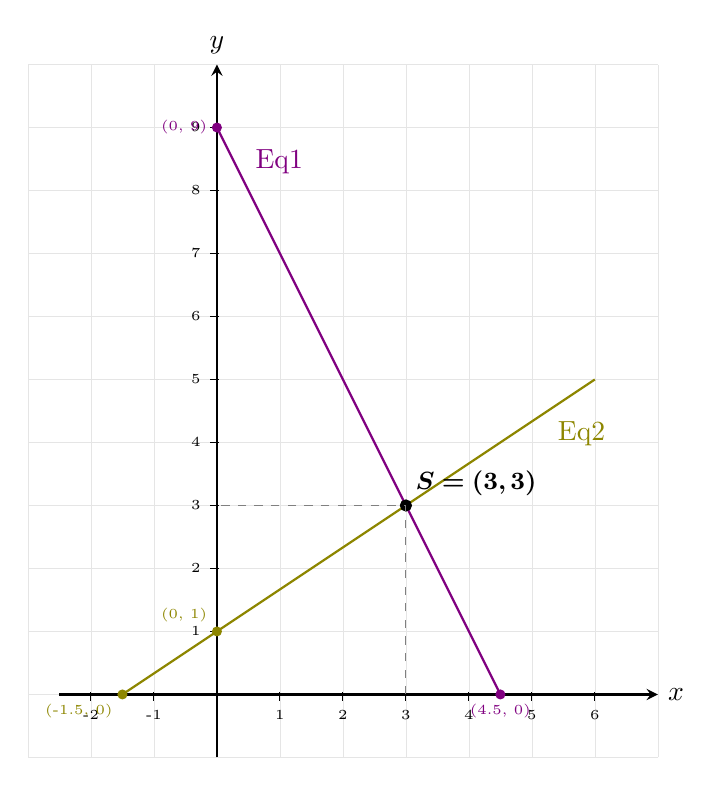
\begin{tikzpicture}[scale=0.8, >=stealth]
    \draw[very thin, gray!20] (-3,-1) grid (7,10);

    \draw[->, thick] (-2.5,0) -- (7,0) node[right] {$x$}; 
    \draw[->, thick] (0,-1) -- (0,10) node[above] {$y$}; 

    \foreach \x in {-2, -1, 1, 2, 3, 4, 5, 6}
        \draw (\x, 1pt) -- (\x, -3pt) node[below, font=\tiny] {\x};
    \foreach \y in {1, 2, 3, 4, 5, 6, 7, 8, 9}
        \draw (1pt, \y) -- (-3pt, \y) node[left, font=\tiny] {\y};

    \draw[violet, thick] (0,9) -- (4.5,0) node[above right, pos=0.1] {Eq1};
    \filldraw[violet] (0,9) circle (2pt) node[left, font=\tiny] {(0, 9)};
    \filldraw[violet] (4.5,0) circle (2pt) node[below, font=\tiny] {(4.5, 0)};

    \draw[olive, thick] (-1.5,0) -- (6,5) node[below right, pos=0.9] {Eq2}; 
    \filldraw[olive] (0,1) circle (2pt) node[above left, font=\tiny] {(0, 1)};
    \filldraw[olive] (-1.5,0) circle (2pt) node[below left, font=\tiny] {(-1.5, 0)};

    \filldraw[black] (3,3) circle (2.5pt);
    \draw[dashed, gray] (3,0) -- (3,3) -- (0,3);
    \node[above right, font=\small] at (3,3) {$\bm{S = (3, 3)}$};

\end{tikzpicture}
%b)
\subsubsection*{b) Determine x e y.}
$x =3, y= 3$\\
% Questão 7
\subsubsection*{7. Considere o sistema:}

\begin{equation*}
\begin{cases}
    x + 2y = 5 \\
    3x + 4y = 11
\end{cases}
\end{equation*}
%a)
\subsubsection*{a) Escreva o sistema na forma matricial Ax = b.}
$$
\begin{bmatrix}
    1 & 2\\
    3 & 4
\end{bmatrix}
\begin{bmatrix}
    x \\
    y
\end{bmatrix}
=
\begin{bmatrix}
    5 \\
    11
\end{bmatrix}
$$
%b)
\subsubsection*{b) Monte a matriz aumentada.}
\[
\left[
\begin{array}{cc|c}
  1 & 2 & 5 \\
 3 & 4 & 11
\end{array}
\right]
\]
%c)
\subsubsection*{c) Resolva utilizando o método de Gauss (escalonamento).}
$\circulo{1.1}$ Matriz aumentada:\\
\[
\left[
\begin{array}{cc|c}
  1 & 2 & 5 \\
 3 & 4 & 11
\end{array}
\right]
\]\\
$\rightarrow$ Pivô = 1 / Alvo para zerar = 3 $\therefore$ Fator = Alvo $\div$ Pivô $\rightarrow$ $3 \div 1 = \bm{3}$\\\\
$\circulo{1.2}$ Operação para zerar o alvo: $L_2 = L_2 - 3 \times L_1$\\\\
$\circulo{1.3}$ Calculando a segunda linha da matriz:\\
$L_2 = 3 - 3 \times 1 = 0$\\
$L_2 = 4 - 3 \times 2 = -2$\\
$L_2 = 11 - 3 \times 5 = -4$\\
$\circulo{1.3.1}$ Nova matriz:\\
\[
\left[
\begin{array}{cc|c}
  1 & 2 & 5 \\
 0 & -2 & -4
\end{array}
\right]
\]\\
$\circulo{1.4}$ Agora, encontra-se o $\bm{y}$:\\\\
$-2y = -4$\\
$y = \frac{-4}{-2} \rightarrow \bm{y=2}$\\\\
$\circulo{1.5}$ Por fim, o $\bm{x}$:\\
$x + 2 = 5$\\
$x + 2 \times 2 = 5 \therefore \bm{x = 1}$
%d)
\subsubsection*{d) Apresente a solução final.}
$S=\{1,2\}$
% Questão 8
\subsubsection*{8. Considere o sistema:}

\begin{equation*}
    \begin{cases}
        2x + 4y = 6\\
        x + 2y = 3
    \end{cases}
\end{equation*}
%a)
\subsubsection*{a) Resolva o sistema.}
Multiplicando a $Eq_2$ por $-2$ e resolvendo por $\underline{\text{adição}}$:
$$
\begin{matrix}
    2x + 4y = 6 \\
    -2x - 4y = -6 \\ \hline 
    0 = 0 \\ 
\end{matrix}
$$
%b)
\subsubsection*{b) O que ocorre durante o processo de resolução?}
No processo de adição do sistema, o resultado é igual a $\underline{zero}$ na adição de todas as variáveis de ambas as equações. Isso ocorre porque a Equação 1 é apenas a informação $\underline{\text{multiplicada por dois}}$ da Equação 2 ($Eq_1 = 2 \times Eq_2$), ou seja, as equações do sistema têm exatamente as mesmas informações. Assim, o determinante resulta em $\underline{zero}$.
%c)
\subsubsection*{c) Classifique o sistema (solução única, infinitas soluções ou nenhuma solução).}
Infinitas soluções possíveis (SPI $\rightarrow$ Sistema Possível e Indeterminado).
%d)
\subsubsection*{d) Desenhe o gráfico correspondente.}
\begin{center} 
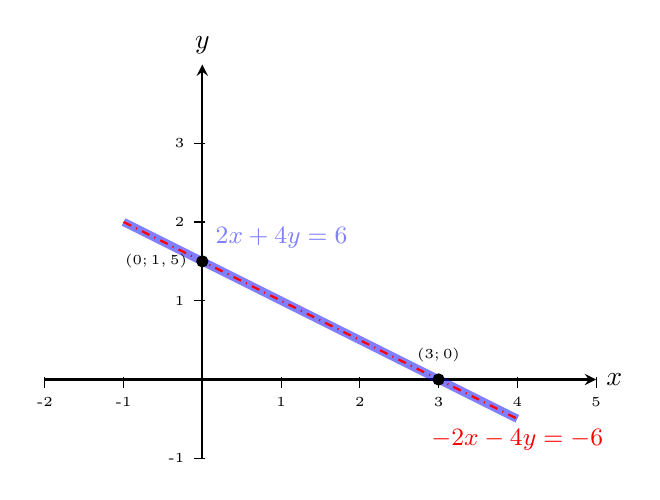
\begin{tikzpicture}[scale=1, >=stealth] 
    % eixos cartesianos
    \draw[->, thick] (-2,0) -- (5,0) node[right] {$x$}; % eixo x
    \draw[->, thick] (0,-1) -- (0,4) node[above] {$y$}; % eixo y

    \foreach \x in {-2, -1, 1, 2, 3, 4, 5}
        \draw (\x, 1pt) -- (\x, -3pt) node[below, font=\tiny] {\x};
    \foreach \y in {-1, 1, 2, 3}
        \draw (1pt, \y) -- (-3pt, \y) node[left, font=\tiny] {\y};
    
    % reta da equação 1 
    \draw[blue, line width=3pt, opacity=0.5] (-1,2) -- (4,-0.5) 
        node[above right, pos=0.2, font=\small] {$2x+4y=6$};
        
    % reta da equação 2 
    \draw[red, dash dot, thick] (-1,2) -- (4,-0.5)
        node[below, pos=1, font=\small] {$-2x-4y=-6$};

    % intersecção das retas
    \filldraw[black] (0,1.5) circle (2pt) node[left, font=\tiny, xshift=-2pt] {$(0; 1,5)$};
    \filldraw[black] (3,0) circle (2pt) node[below, font=\tiny, yshift=15pt] {$(3; 0)$};

\end{tikzpicture}
\end{center}
%e)
\subsubsection*{e) Explique em uma frase objetiva o significado desse resultado.}
 Frase: o sistema possui infinitas soluções porque as duas equações que o compõe são iguais, isto é, a equações representam a mesma reta no plano cartesiano\\
 Colocando a frase em um exemplo: se isso fosse aplicado em uma situação real, por exemplo: duas planilhas de dados dos gastos de uma empresa em um trimestre, com dois tipos de atributos ($Eq1$ para despesas operacionais e $Eq2$ para despesas tributárias), os dados sobre os gastos estariam incorretos e as informações financeiras estariam perdidas. O $\underline{\text{erro}}$ nesse tipo de problema já pode ser encontrado prontamente ao perceber que o determinante desse sistema será igual a $\underline{\text{zero}}$.
% Questão 9
 \subsubsection*{9. Sistema 3×3 (Gauss)}
 \subsubsection*{Resolva o sistema abaixo usando escalonamento de Gauss:}
 \begin{equation*}
\begin{cases}
    x + y + z = 6 \\
    2x + y + z = 9 \\
    x + 2y + 3z = 14
\end{cases}
\end{equation*}
%a)
\subsubsection*{a) Escreva a matriz aumentada.}
$$
\left[
\begin{array}{ccc|c}
    1 & 1 & 1 & 6 \\
    2 & 1 & 1 & 9 \\
    1 & 2 & 3 & 14
\end{array}
\right]
$$
%b)
\subsubsection*{b) Realize o escalonamento.}
$\circulo{1}$ Fator: 2\\
$\circulo{1.2}$ Para zerar a linha 2, coluna 1: $L_2 = L_2-2 \times L_1$\\
$\circulo{1.3}$ Cálculos da $L_2$:\\
$L_2 = 2 - 2 \times 1 = 0$\\
$L_2 = 1 - 2 \times 1 = -1$\\
$L_2 = 1 - 2 \times 1 = -1$\\
$L_2 = 9 - 2 \times 6 = -3$\\\\
$\circulo{1.4}$ Agora, zera-se a linha 3, coluna 1:\\
Fator: 1\\
Para zerar a linha 3, coluna 1: $L_3 = L_3 - L_1$\\
$\circulo{1.5}$ Cálculos da $L_3$:\\ 
$L_3 = 1 - 1= 0$\\
$L_3 = 2 - 1 = 1$\\
$L_3 = 3- 1 = 2$\\
$L_3 = 14 - 6 = 8$\\\\
$\circulo{1.6}$ Matriz atualizada:

$$
\left[
\begin{array}{ccc|c}
    1 & 1 & 1 & 6 \\
    0 & -1 & -1 & -3 \\
    0 & 1 & 2 & 8
\end{array}
\right]
$$

$\circulo{2}$ Agora, é preciso zerar o elemento na linha 3, coluna 2:\\
Fator: -1\\
Para zerar a linha 3, coluna 2: $L_3 = L_3 + L_2$\\\\
$\circulo{2.1}$ Cálculos da $L_3$:\\
$L_3 = 0 + 0 = 0$\\
$L_3 = 1 + (-1) = 0$\\
$L_3 = 2 + (-1) = 1$\\
$L_3 = 8 + (-3) = 5$\\\\
$\circulo{3}$ Matriz escalonada:\\
$$
\left[
\begin{array}{ccc|c}
    1 & 1 & 1 & 6 \\
    0 & -1 & -1 & -3 \\
    0 & 0 & 1 & 5
\end{array}
\right]
$$
%c)
\subsubsection*{c) Apresente a solução (x,y,z).}
$1z = 5 \therefore \fbox{z = 5}$\\
$0 - y - 5 = -3 \rightarrow -y = 2 \therefore \fbox{y = -2}$\\
$x - 2 + 5 = 6 \rightarrow x= 6 - 3 \therefore \fbox{x = 3}$\\\\
S = \{ 3, -2, 5\}
% Questão 10
\subsubsection*{10. Questão de sala de aula (MATRIZES)}
\subsubsection*{Uma equipe de pesquisa está analisando 4 unidades de saúde quanto ao uso de
dados e tecnologia em suas rotinas.\\
Foram definidos dois indicadores (normalizados entre 0 e 10):\\
X1: Grau de digitalização de prontuários\\
X2: Uso de dados para tomada de decisão\\
A matriz de dados é:}
\begin{table}[h]
\centering
\begin{tabular}{|c|c|c|}
\hline
\textbf{Unidade} & \textbf{X1} & \textbf{X2} \\ \hline
U1               & 2           & 1           \\ \hline
U2               & 3           & 3           \\ \hline
U3               & 7           & 6           \\ \hline
U4               & 8           & 2           \\ \hline
\end{tabular}
\end{table}
Cada unidade é representada por um vetor em $\mathbb{R}^2$:\\
$U1 = (2, 1)$\\
$U2 = (3, 3)$\\
$U3 = (7, 6)$\\
$U4 = (8, 2)$

\subsubsection*{Pede-se:\\
– Calcule a distância Euclidiana entre todos os pares de unidades\\
– Monte a matriz de distâncias\\
– Realize o agrupamento hierárquico usando complete linkage (ligação completa)\\
– Esboce o dendrograma\\
– Considere um corte que gere dois grupos e interprete o resultado.\\}
$\circulo{1}$ Cálulo da distância Euclidiana:\\
$\underset{1,2}{U} = \sqrt{(2-3)^2 + (1-3)^2} = \sqrt{1+4} = \sqrt{5} = \bm{2,24}\\$
$\underset{1,3}{U} = \sqrt{(2-7)^2 + (1-6)^2} = \sqrt{25+25} = \sqrt{50} = \bm{7,07}\\$
$\underset{1,4}{U} = \sqrt{(2-8)^2 + (1-2)^2} = \sqrt{36+1} = \sqrt{37} = \bm{6,08}\\$
$\underset{2,3}{U} = \sqrt{(3-7)^2 + (3-6)^2} = \sqrt{16+9} = \sqrt{25} = \bm{5}\\$
$\underset{2,4}{U} = \sqrt{(3-8)^2 + (3-2)^2} = \sqrt{25+1} = \sqrt{26} = \bm{5,09}\\$
$\underset{3,4}{U} = \sqrt{(7-8)^2 + (6-2)^2} = \sqrt{1+16} = \sqrt{17} = \bm{4,12}\\\\$
$\circulo{2}$ Matriz de distâncias:

\renewcommand{\arraystretch}{1.5}
$$
\begin{tabular}{|c|c|c|c|c|}
    \hline
    & $U1$ & $U2$ & $U3$ & $U4$ \\ \hline
    $U1$ & 0     & 2,24  & 7,07  & 6,08  \\ \hline
    $U2$ & 2,24  & 0     & 5  & 5,09  \\ \hline
    $U3$ & 7,07  & 5  & 0     & 4,12  \\ \hline
    $U4$ & 6,08  & 5,09  & 4,12  & 0     \\ \hline
\end{tabular}
$$\\

$\circulo{3}$ Agrupamento hierárquico com complete linkage:\\
$\rightarrow$ Escolha do par mais próximo (menor distância):\\
$(U1, U2)$ | Altura no dendograma: $2,24$\\\\
$\circulo{4}$ Atualização da matriz com o cálculo entre a distância do agrupamento (U1, U2) e as distâncias U3 e U4:\\\\
$\bullet$ Distância de (U1, U2) até U3:\\
$d((U1, U2), U3) = max(d(U1, U3), d(U2,U3)) = max(7,07; 5) = \bm{7,07}$\\\\
$\bullet$ Distância de (U1, U2) até U4:\\
$d((U1, U2), U4) = max(d(U1, U4), d(U2, U4)) = max(6,08; 5,09)
 = \bm{6,08}$\\\\
 $\circulo{4.1}$ Nova matriz:
\renewcommand{\arraystretch}{1.5}
$$
\begin{tabular}{|c|c|c|c|}
    \hline
    & $(U1, U2)$ & $U3$ & $U4$ \\ \hline
    $(U1, U2)$ & 0  & 7,07  & 6,08  \\ \hline
    $U3$ & 7,07  & 0     & 4,12  \\ \hline
    $U4$ & 6,08 & 4,12  & 0     \\ \hline
\end{tabular}
$$\\\\
$\circulo{5}$ Segunda iteração:\\ 
$\circulo{5.1}$ Escolha do par mais próximo (menor distância):\\
$(U3, U4)$ | Altura no dendograma: $4,12$\\\\

$\circulo{5.2}$ Cálculo das distâncias entre (U1, U2) e (U3, U4):\\
$d((U1, U2), (U3, U4)) = max(d((U1, U2), U3), d((U1, U2), U4)) = max(7,07; 6,08) = \bm{7,07}$\\\\
$\circulo{5.3}$ Matriz atualizada:

\renewcommand{\arraystretch}{1.5}
$$
\begin{tabular}{|c|c|c|}
    \hline
    & $(U1, U2)$ & $(U3, U4)$  \\ \hline
    $(U1, U2)$ & 0  & 7,07  \\ \hline
    $(U3, U4)$ & 7,07  & 0 \\ \hline
\end{tabular}
$$

$\circulo{6}$ Terceira iteração - apenas uma distância:\\
Distância entre (U1, U2) e (U3, U4) = $\bm{7,07}$, e também é a altura dos dois agrupamentos no dendograma.\\\\
$\circulo{7}$  Esboce o dendrograma.

\begin{tikzpicture}[yscale=1.2, xscale=1.2]
    \draw[->, thick] (0,0) -- (0,8) node[above] {Distância};
    \draw[->, thick] (0,0) -- (6,0) node[below] {Unidades};

    % eixo x em 10^-3
    \foreach \y in {0, 1, 2, 3, 4, 5, 6, 7, 8}
        \draw (1pt,\y) -- (-3pt,\y) node[left, font=\small] {\y};

    \draw (1,0) node[below] {$U_1$} -- (1,2.24);
    \draw (2,0) node[below] {$U_2$} -- (2,2.24);
    \draw (1,2.24) -- (2,2.24) node[right, above] {{2,24}};

    \draw (4,0) node[below] {$U_3$} -- (4,4.12);
    \draw (5,0) node[below] {$U_4$} -- (5,4.12);
    \draw (4,4.12) -- (5,4.12) node[left, above] {4,12};

    \draw (1.5,2.24) -- (1.5,7.07);
    \draw (4.5,4.12) -- (4.5,7.07);
    \draw (1.5,7.07) -- (4.5,7.07) node[midway, above] {{7,07}};

\end{tikzpicture}
\\\\
$\circulo{8}$ Considere um corte que gere dois grupos e interprete o resultado.\\
É possível gerar dois grups em um corte na distância $\bm{6}$, por exemplo. Observa-se, primeiramente, que U1 e U2 usam os dados e digitalizam prontuários de forma bem semelhante, mas o uso de tecnologias por essas unidades de saúde ainda é baixo($2,24$). Por outro lado, as unidades U3 e U4 utilizam a tecnologia de forma bastante similar entre si e com maior frequência do que o agrupamento (U3, U4) ($4,12$). Aqui, pode-se concluir que um possível incentivo ao uso da tecnologia em USs deve ser reforçado em U1 e U2, e melhorado, mas não com tanta urgência, em U3 e U4.

% Questão 11 - extra
\subsubsection*{11. QUESTÃO EXTRA (SISTEMAS LINEARES)}
\subsubsection*{Problema 1: O Data Center\\
Você é gerente de infraestrutura de uma startup. Vocês alugam servidores na nuvem de três tipos: Básico (x), Standard (y) e Premium (z). O
financeiro perdeu o contrato com os preços unitários, mas temos as notas fiscais totais de três departamentos.\\
O Sistema (Recursos Consumidos):\\
• Eq 1 (Quantidade): O total de máquinas alugadas foi 17.\\
• Eq 2 (Memória RAM): O consumo total d e RAM foi 56 GB.\\
• Eq 3 (Armazenamento): O consumo total de HD foi 35 TB.\\}
$$
\begin{cases}
    x + y + z = 17 \\
    2x + 4y + 8z = 56 \\
    x + 3y + 5z = 35
\end{cases}
$$\\
\subsubsection*{Sua Missão: Descubra quantos servidores de cada tipo (X, Y, Z) a empresa possui.}

$\circulo{1}$ Matriz inicial:
\[
\left[
\begin{array}{ccc|c}
    \bm{1} & 1 & 1 & 17 \\
    2 & 4 & 8 & 56 \\
    1 & 3 & 5 & 35
\end{array}
\right]
\begin{array}{l}
    \leftarrow \text{Pivô} \\
    \text{Fator: } 2/1 = 2 \\
    \text{Fator: } 1/1 = 1
\end{array}
\]

$\circulo{2}$ Zerar a coluna 1:
\begin{itemize}
    \item $L_2 \leftarrow L_2 - 2 \cdot L_1$
    \begin{itemize}
        \item $2 - 2 \cdot 1 = 0$
        \item $4 - 2 \cdot 1 = 2$
        \item $8 - 2 \cdot 1 = 6$
        \item $56 - 2 \cdot 17 = 56 - 34 = 22$
    \end{itemize}
    \item $L_3 \leftarrow L_3 - 1 \cdot L_1$
    \begin{itemize}
        \item $1 - 1 \cdot 1 = 0$
        \item $3 - 1 \cdot 1 = 2$
        \item $5 - 1 \cdot 1 = 4$
        \item $35 - 1 \cdot 17 = 18$
    \end{itemize}
\end{itemize}

Nova matriz:
\[
\left[
\begin{array}{ccc|c}
    1 & 1 & 1 & 17 \\
    0 & \bm{2} & 6 & 22 \\
    0 & 2 & 4 & 18
\end{array}
\right]
\begin{array}{l}
    \\
    \leftarrow \text{Novo Pivô} \\
    \text{Fator: } 2/2 = 1
\end{array}
\]

$\circulo{3}$Zerar a coluna 2:
\begin{itemize}
    \item $L_3 \leftarrow L_3 - 1 \cdot L_2$
    \begin{itemize}
        \item $0 - 0 = 0$
        \item $2 - 2 = 0$
        \item $4 - 6 = -2$
        \item $18 - 22 = -4$
    \end{itemize}
\end{itemize}

$\circulo{4}$ Matriz escalonada:
\[
\left[
\begin{array}{ccc|c}
    1 & 1 & 1 & 17 \\
    0 & 2 & 6 & 22 \\
    0 & 0 & -2 & -4
\end{array}
\right]
\]

$\circulo{5}$ Encontrar os valores de x, y e z:
\begin{itemize}
    \item \textbf{Cálculo de $z$:}
    \[ -2z = -4 \therefore \bm{z = 2} \]
    \item \textbf{Cálculo de $y$:}
    \[ 2y + 6z = 22 \]
    \[ 2y + 6(2) = 22 \rightarrow 2y + 12 = 22 \rightarrow 2y = 10 \therefore \bm{y = 5} \]
    \item \textbf{Cálculo de $x$:}
    \[ x + y + z = 17 \]
    \[ x + 5 + 2 = 17 \rightarrow x + 7 = 17 \therefore \bm{x = 10} \]
\end{itemize}

\[ S = \{10, 5, 2\} \]

\subsubsection*{Problema 2: Consultoria de BI}
\subsubsection*{Uma empresa de Business Intelligence cobra por hora de analistas: Júnior ($x$), Pleno ($y$) e Sênior ($z$). Temos os registros de horas e
faturamento de três projetos, mas precisamos isolar quanto cada nível de senioridade trabalhou.\\\\
O Sistema:}
$$
\begin{cases}
    x + y + z = 35 & \text{(Total de horas no Projeto A)} \\
    2x + 3y + z = 75 & \text{(Total de horas no Projeto B)} \\
    x + 2y + 3z = 55 & \text{(Total de horas no Projeto C)}
\end{cases}
$$\\
\subsubsection*{Sua Missão: Descubra quantas horas foram dedicadas por cada nível (x, y , z).}


\[
\begin{cases}
    x + y + z = 35 \\
    2x + 3y + z = 75 \\
    x + 2y + 3z = 55
\end{cases}
\]

$\circulo{1}$ Matriz aumentada:
\[
\left[
\begin{array}{ccc|c}
    \textcircled{1} & 1 & 1 & 35 \\
    2 & 3 & 1 & 75 \\
    1 & 2 & 3 & 55
\end{array}
\right]
\begin{array}{l}
    \leftarrow \text{Pivô} \\
    \\
    \\
\end{array}
\]

$\circulo{1.1}$ Zerar o 2 (alvo da 2ª linha):\\
Fator $= \frac{\text{Alvo}}{\text{Pivô}} = \frac{2}{1} = \textcircled{2} \therefore L_2 = L_2 - 2 \cdot L_1$

\begin{itemize}
    \item $L_2 = 2 - 2 \cdot 1 = 0$
    \item $L_2 = 3 - 2 \cdot 1 = 1$
    \item $L_2 = 1 - 2 \cdot 1 = -1$
    \item $L_2 = 75 - 2 \cdot 35 = 5$
\end{itemize}

\[
\rightarrow \left[
\begin{array}{ccc|c}
    1 & 1 & 1 & 35 \\
    \textcircled{0} & 1 & -1 & 5 \\
    1 & 2 & 3 & 55
\end{array}
\right]
\begin{array}{l}
    \\
    \\
\end{array}
\]

$\circulo{1.2}$ Zerar o 1 (alvo da 3ª linha):\\
Fator $= \text{Alvo/Pivô} = 1/1 = \textcircled{1} \therefore L_3 = L_3 - 1 \cdot L_1$

\begin{itemize}
    \item $L_3 = 1 - 1 = 0$
    \item $L_3 = 2 - 1 = 1$
    \item $L_3 = 3 - 1 = 2$
    \item $L_3 = 55 - 35 = 20$
\end{itemize}

\[
\rightarrow \left[
\begin{array}{ccc|c}
    1 & 1 & 1 & 35 \\
    0 & 1 & -1 & 5 \\
    \textcircled{0} & 1 & 2 & 20
\end{array}
\right]
\begin{array}{l}
    \\
    \\
\end{array}
\]

$\circulo{1.3}$ Zerar o 1 (alvo da 3ª coluna):\\
Fator $= \text{Alvo/Pivô} = 1/1 = \textcircled{1} \therefore L_3 = L_3 - L_2$

\begin{itemize}
    \item $L_3 = 0 - 0 = 0$
    \item $L_3 = 1 - 1 = 0$
    \item $L_3 = 2 + 1 = 3$
    \item $L_3 = 20 - 5 = 15$
\end{itemize}

\[
\circulo{1.4} \text{ Matriz escalonada:}
\]
\[
\]
\[
\left[
\begin{array}{ccc|c}
    1 & 1 & 1 & 35 \\
    0 & 1 & -1 & 5 \\
    0 & 0 & 3 & 15
\end{array}
\right]
\]

$\circulo{2}$ Resolve a equação da linha 3 (para z):\\
$3z = 15 \therefore z = 5$\\\\

$\circulo{2.1}$ Resolve a equação da linha 2 (para y):\\
$y - 5 = 5 \therefore y = 10$\\\\

$\circulo{2.2}$ Resolve a equação da linha 1 (para x):\\
$x + 10 + 5 = 35$\\
$x = 35 - 15 \therefore x= 20$\\\\

$S = \{20, 10, 5\}$
\end{document}
